\documentclass[12pt,a4paper]{article}

\usepackage[utf8]{inputenc}
\usepackage[T1]{fontenc}
\usepackage[brazilian]{babel}
\usepackage{lmodern}
\usepackage{geometry}
\usepackage{microtype}
\usepackage{graphicx}
\usepackage{float}
\usepackage{booktabs}
\usepackage{longtable}
\usepackage{array}
\usepackage{amsmath}
\usepackage{siunitx}
\usepackage{caption}
\usepackage{subcaption}
\usepackage{circuitikz}
\usetikzlibrary{decorations.pathreplacing}
\usepackage{animate}
\usepackage{cite}
\usepackage{url}
\usepackage[colorlinks=true,linkcolor=blue,citecolor=blue,urlcolor=blue]{hyperref}

\geometry{margin=2.5cm}
\graphicspath{{figures/output/}{figures/}{frames/}}
\sisetup{
  detect-all,
  per-mode=symbol,
  exponent-product=\cdot,
  output-decimal-marker={.}
}
\setlength{\parskip}{0.55em}
\setlength{\parindent}{0pt}
\captionsetup{font=small,labelfont=bf}

\newcommand{\projectpath}{\texttt{E:\textbackslash surto-1}}
\newcommand{\reportpath}{\texttt{E:\textbackslash surto-1\textbackslash relatorio}}
\newcommand{\codefile}[1]{\texttt{#1}}
\newcommand{\Nsec}{20}
\newcommand{\Rsec}{\ensuremath{R_{\mathrm{sec}}}}
\newcommand{\Lsec}{\ensuremath{L_{\mathrm{sec}}}}
\newcommand{\Csec}{\ensuremath{C_{\mathrm{sec}}}}
\newcommand{\Vsrc}{\ensuremath{v_s(t)}}
\newcommand{\Zsurge}{\ensuremath{Z_0}}
\newcommand{\Ttravel}{\ensuremath{T_{\mathrm{prop}}}}

\newcommand{\staticfigure}[4]{
  \begin{figure}[H]
    \centering
    \includegraphics[width=#1\linewidth]{#2}
    \caption{#3}
    \label{#4}
  \end{figure}
}


\title{Distribuição de tensão de surto no enrolamento de um gerador síncrono}
\author{Projeto \texttt{surto-1}}
\date{\today}

\begin{document}

\maketitle
\tableofcontents
\listoffigures
\clearpage

\section{Resumo}

Este relatório descreve \emph{como a tensão de um surto se distribui ao longo do enrolamento de um
gerador síncrono} com o neutro solidamente aterrado. Quando uma frente de onda rápida — o impulso
atmosférico padrão \SI{1.2}{\micro\second}/\SI{50}{\micro\second} — atinge a entrada da máquina, o
enrolamento não responde como uma única indutância concentrada: no primeiro instante ele se comporta
como uma \emph{rede capacitiva}, e a tensão se concentra de forma acentuada nas primeiras espiras.

O enrolamento é representado por uma escada de \Nsec{} seções com resistência e indutância série
(\Rsec, \Lsec), capacitância para o núcleo aterrado (\Cg, \emph{shunt}) e capacitância entre espiras
(\Cs, \emph{série}). A razão entre as duas capacitâncias define o parâmetro de distribuição
\(\adist = \sqrt{\Cg/\Cs}\), que controla quão desigual é a repartição inicial da tensão. Para a
máquina estudada adota-se \(\adist = 5\).

A história física tem dois instantes-chave. Em \(t = 0^+\), a distribuição é capacitiva e fortemente
não uniforme, \(v(x)/V_0 = \sinh\!\big(\adist(1-x)\big)/\sinh(\adist)\), com a entrada solicitada por
um fator \(\adist\coth\adist \approx 5\) acima da média. Depois, a indutância entra em ação e a
distribuição relaxa para um perfil quase uniforme, preso a zero no neutro aterrado. É essa
\emph{transição do perfil concentrado para o uniforme} que dimensiona o isolamento de entrada e que
este relatório documenta, com animações geradas a partir da simulação. Os resultados foram validados
contra a solução analítica clássica de surtos em enrolamentos \cite{greenwood1991} e por uma simulação
independente em ATP/EMTP \cite{dommel1969}.

\section{Visão geral do projeto}

O projeto implementa um simulador de resposta a surto em bobina distribuída. A ideia central é substituir o enrolamento contínuo por uma cadeia de seções concentradas, cada uma contendo resistência, indutância e capacitância para terra. Essa discretização permite estudar fenômenos de alta frequência que um modelo puramente concentrado perderia, como atraso de propagação, reflexões na extremidade aberta e distribuição não uniforme de tensão.

A pasta \codefile{config} contém o caso base em \codefile{default\_case.json}. A pasta \codefile{src} contém o modelo elétrico, a fonte, o solver, o processamento de resultados e a visualização. A pasta \codefile{output} contém os CSVs, PNGs e GIFs já gerados. O arquivo \codefile{surto\_bobina.atp} descreve um caso ATP com a mesma lógica física do modelo Pi: \Nsec{} ramos série R--L, capacitores shunt para terra e uma fonte dupla exponencial aplicada no nó de entrada.

Os resultados numéricos são exportados como tensões nodais, correntes de seção e um resumo com picos de tensão e gradientes. Os resultados visuais incluem curvas de entrada/saída, curvas em nós selecionados, mapas de calor posição-tempo, barras de pico por nó, barras de gradiente entre nós adjacentes e animações da onda viajante.

\begin{table}[H]
\centering
\caption{Parâmetros principais do caso padrão em \codefile{config/default\_case.json}.}
\label{tab:parametros-caso}
\begin{tabular}{lll}
\toprule
Parâmetro & Valor & Interpretação elétrica \\
\midrule
\codefile{n\_sections} & 20 & número de seções discretas \\
\codefile{L\_total} & \SI{0.01}{H} & indutância total da bobina \\
\codefile{R\_total} & \SI{5}{\ohm} & perdas série totais \\
\codefile{C\_total} & \SI{1e-9}{F} & capacitância total para terra \\
\codefile{model\_type} & \codefile{pi} & topologia Pi principal \\
\codefile{source\_type} & \codefile{double\_exp} & impulso dupla exponencial \\
\codefile{V\_amplitude} & \SI{1000}{V} & pico nominal da fonte \\
\codefile{t\_front} & \SI{1.2}{\micro\second} & tempo de frente \\
\codefile{t\_tail} & \SI{50}{\micro\second} & tempo de cauda \\
\codefile{dt} & \SI{10}{ns} & passo de amostragem dos resultados \\
\codefile{termination} & \codefile{open} & extremidade aberta \\
\bottomrule
\end{tabular}
\end{table}

\section{A fonte de surto (1,2/50\,\texorpdfstring{$\mu$}{u}s)}
\label{sec:fonte}

A excitação é o impulso atmosférico padrão, modelado por uma dupla exponencial:

\begin{equation}
\Vsrc = V_{\mathrm{pico}}\,K\left(e^{-a t} - e^{-b t}\right), \qquad t \ge 0,
\end{equation}

em que \(a = \ln(2)/T_2\) controla a cauda e \(b = 3/T_1\) controla a frente. Para
\(T_1 = \SI{1.2}{\micro\second}\) (tempo de frente) e \(T_2 = \SI{50}{\micro\second}\) (tempo de cauda),
tem-se \(a \approx \SI{1.3863e4}{s^{-1}}\) e \(b \approx \SI{2.5e6}{s^{-1}}\); a constante \(K\)
normaliza o pico para \(V_{\mathrm{pico}} \approx \SI{1}{kV}\). É a forma clássica de ensaio de impulso
de alta tensão \cite{kuffel2000,iec60060}.

O que torna esse surto crítico para um enrolamento não é a amplitude, e sim a \emph{frente rápida}: os
\SI{1.2}{\micro\second} de subida injetam um espectro de alta frequência que enxerga o enrolamento como
uma rede capacitiva. É essa frente que produz a distribuição inicial não uniforme analisada nas seções
seguintes; a cauda de \SI{50}{\micro\second} apenas sustenta a tensão enquanto a redistribuição
interna ocorre.

\section{Modelo elétrico da bobina distribuída}

Em baixas frequências, uma bobina pode ser aproximada por uma indutância e uma resistência equivalentes. Em um surto rápido, essa simplificação é limitada: a capacitância do enrolamento para terra e a distribuição espacial de indutância e resistência passam a determinar como a tensão se reparte ao longo da bobina. Por isso o projeto usa uma aproximação de parâmetros distribuídos, semelhante ao tratamento de linhas por seções discretas \cite{greenwood1991}.

No caso base, os parâmetros totais são divididos em \Nsec{} seções:

\begin{align}
R_{\mathrm{sec}} &= \frac{R_{\mathrm{total}}}{N} = \frac{5}{20} = \SI{0.25}{\ohm},\\
L_{\mathrm{sec}} &= \frac{L_{\mathrm{total}}}{N} = \frac{0.01}{20} = \SI{0.5}{mH},\\
C_{\mathrm{sec}} &= \frac{C_{\mathrm{total}}}{N} = \frac{10^{-9}}{20} = \SI{50}{pF}.
\end{align}

Na topologia Pi, os capacitores de extremidade aparecem como \(\Csec/2\), enquanto os nós internos possuem \(\Csec\), resultado da soma das duas meias capacitâncias das seções vizinhas. A Figura~\ref{fig:circuito-pi} mostra essa representação.

\begin{figure}[H]
\centering
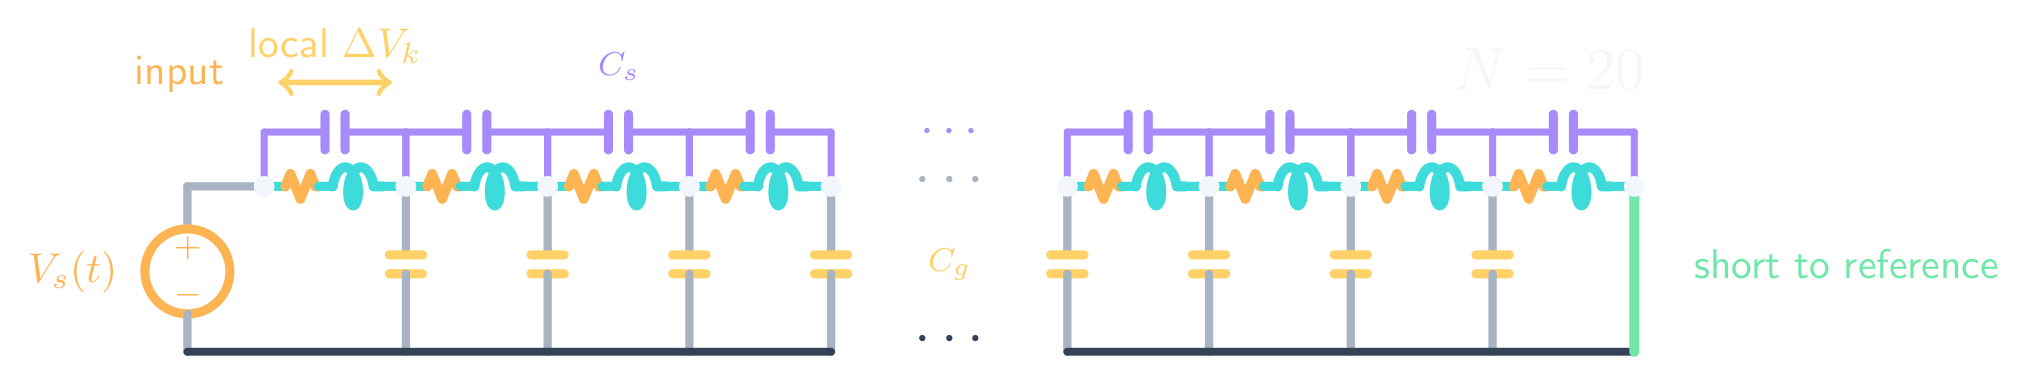
\includegraphics[width=\linewidth]{circuito_grounded.png}
\caption{Escada equivalente do enrolamento. Cada seção tem um ramo série \(R\text{--}L\), uma
capacitância série entre espiras \(\Cs\) (\emph{turn-to-turn}, em roxo, arqueada sobre o ramo) e uma
capacitância shunt para o núcleo aterrado \(\Cg\) (em amarelo). A fonte de surto \(\Vsrc\) entra à
esquerda; o neutro (terminal final) é \emph{solidamente aterrado}. É o mesmo circuito da apresentação
animada e da validação cruzada em ATP.}
\label{fig:circuito-pi}
\end{figure}


Do ponto de vista físico, o ramo \(R-L\) armazena energia magnética e dissipa parte dela em resistência, enquanto o capacitor para terra armazena energia elétrica. A interação entre esses armazenamentos faz com que a perturbação de tensão não apareça instantaneamente em toda a bobina: ela se propaga como onda. A impedância de surto aproximada do conjunto é:

\begin{equation}
\Zsurge = \sqrt{\frac{L_{\mathrm{total}}}{C_{\mathrm{total}}}}
       = \sqrt{\frac{0.01}{10^{-9}}}
       \approx \SI{3162}{\ohm}.
\end{equation}

Uma estimativa de tempo de propagação associada ao par \(L_{\mathrm{total}}, C_{\mathrm{total}}\) é:

\begin{equation}
\Ttravel = \sqrt{L_{\mathrm{total}}C_{\mathrm{total}}}
         = \sqrt{0.01\cdot 10^{-9}}
         \approx \SI{3.16}{\micro\second}.
\end{equation}

A saída está em circuito aberto. Para uma onda incidente, essa condição implica corrente terminal nula e tende a produzir reflexão de tensão com mesmo sinal. A duplicação aproximada do pico na extremidade aberta é coerente com os resultados numéricos: a tensão de entrada atinge \SI{1000}{V}, enquanto a saída chega a cerca de \SI{2039}{V}. Esse valor não é uma simples regra ideal, porque a rede discreta, a resistência e a forma temporal do impulso modificam a resposta.

O modelo T, também implementado no projeto, desloca a capacitância de cada seção para um ponto intermediário. Em termos de engenharia, Pi e T são aproximações discretas diferentes de uma mesma estrutura distribuída. A comparação entre eles ajuda a avaliar se a interpretação física depende fortemente da topologia numérica escolhida.

\section{A distribuição inicial e sua evolução}
\label{sec:distribuicao}

\subsection{O instante do surto (\texorpdfstring{$t=0^+$}{t=0+}): divisor capacitivo}

No primeiro instante após a chegada da frente, os indutores bloqueiam a corrente e o enrolamento é uma
rede puramente capacitiva. Resolvendo essa rede com o neutro aterrado, a tensão se distribui segundo a
solução clássica \cite{greenwood1991}:

\begin{equation}
\frac{v(x)}{V_0} = \frac{\sinh\!\big(\adist(1-x)\big)}{\sinh(\adist)},
\qquad x \in [0,1],
\label{eq:sinh}
\end{equation}

em que \(x=0\) é a entrada (energizada) e \(x=1\) é o neutro aterrado. A Figura~\ref{fig:dist-inicial}
mostra esse perfil, calculado pelo \emph{modelo} (não desenhado à mão), para vários valores de
\(\adist\): quanto maior \(\adist\), mais a tensão se acumula nas primeiras seções e mais a curva se
afasta da reta uniforme.

\staticfigure{0.92}{distribuicao_inicial.png}{Distribuição inicial de tensão \(v(x)/V_0\) em
\(t=0^+\), com neutro aterrado, obtida do modelo distribuído (\codefile{initial\_voltage\_distribution})
para \(\adist = 1, 3, 5, 8\). A reta tracejada é a distribuição uniforme ingênua (\(\adist\to 0\)).
Para a máquina estudada, \(\adist=5\).}{fig:dist-inicial}

A não uniformidade é medida pelo \emph{fator de concentração na entrada}, o gradiente local na primeira
espira em relação ao gradiente médio:

\begin{equation}
\left.\frac{\mathrm{d}}{\mathrm{d}x}\frac{v}{V_0}\right|_{x=0}
   = \adist\coth(\adist) \approx \adist = 5 .
\label{eq:concentracao}
\end{equation}

Ou seja: para \(\adist=5\), a primeira fração do enrolamento é solicitada por cerca de \textbf{cinco
vezes} a tensão que veria se a distribuição fosse uniforme. É esse o mecanismo que estressa o isolamento
de entrada de máquinas e transformadores.

\subsection{A evolução no tempo: do perfil concentrado ao uniforme}

A distribuição da Equação~\eqref{eq:sinh} é apenas o ponto de partida. À medida que a corrente começa a
circular pelos indutores, a energia se redistribui e o perfil \emph{relaxa} de uma forma concentrada
para uma distribuição quase uniforme, presa a zero no neutro aterrado. Durante essa transição surgem
oscilações internas e sobretensões: a simulação no tempo indica pico em torno de \SI{1108}{V} no nó a
25\,\% do enrolamento (\(N_5\)) — acima do \SI{1}{kV} aplicado na entrada. A Seção~\ref{sec:animacoes}
mostra essa evolução em animação.

A leitura de engenharia é que o \emph{envelope} de tensão ao longo do enrolamento — e não o regime
permanente — dimensiona o isolamento: as primeiras espiras concentram a solicitação no instante do
surto, e nós internos podem exceder a tensão de entrada durante a redistribuição.

\section{Animacoes em GIF e incorporacao no PDF}

Os GIFs originais em \codefile{output/gifs} foram convertidos para sequencias de frames PNG dentro de \codefile{relatorio/frames}, usando \codefile{ffmpeg}. Nesta revisao, a animacao incorporada ao PDF foi atualizada para o caso Pi com retorno aterrado: a fonte de surto fica entre o no de referencia e a entrada da bobina, e o terminal final da bobina retorna diretamente ao mesmo no de referencia. Assim, a animacao documenta a condicao solicitada de fim da bobina conectado ao no comum com a fonte, em vez de enfatizar apenas a extremidade aberta.

A incorporacao usa o pacote \codefile{animate}. Em visualizadores compativeis, como Adobe Acrobat Reader, as figuras podem ser reproduzidas com controles. Em visualizadores simples, o PDF pode exibir apenas um quadro estatico.

\subsection{Onda viajante com retorno ao no comum}

\begin{figure}[H]
\centering
\animategraphics[controls,loop,autoplay,width=0.90\linewidth]{5}{frames/voltage_wave_grounded/frame-}{1}{75}
\caption{Animacao da distribuicao de tensao ao longo da bobina no modelo Pi com terminal final conectado ao no de referencia. A entrada recebe o surto e a extremidade em 100\% permanece presa ao potencial comum da fonte.}
\label{fig:anim-grounded-wave}
\end{figure}

A Figura~\ref{fig:anim-grounded-wave} mostra que a resposta deixa de ser a mesma do terminal aberto. No caso aberto, a corrente terminal nula favorece reflexao de tensao com mesmo sinal e elevacao da tensao na extremidade. No caso com retorno ao no comum, o terminal final e imposto em \SI{0}{V}; por isso a informacao mais importante passa a ser a distribuicao interna de tensao ao longo do enrolamento.

\subsection{Mapa de calor animado do caso aterrado}

\begin{figure}[H]
\centering
\animategraphics[controls,loop,autoplay,width=0.94\linewidth]{5}{frames/heatmap_grounded/frame-}{1}{75}
\caption{Mapa de calor animado do modelo Pi com terminal final conectado ao no comum com a fonte. O cursor temporal relaciona a distribuicao instantanea com o historico posicao-tempo.}
\label{fig:anim-grounded-heatmap}
\end{figure}

A Figura~\ref{fig:anim-grounded-heatmap} complementa a animacao da onda viajante porque mostra o comportamento no plano tempo--posicao. A borda em 100\% permanece vinculada ao no de referencia, enquanto os nos internos respondem ao impulso aplicado na entrada. Essa visualizacao torna mais direta a comparacao conceitual com o caso aberto: muda-se a condicao de contorno, mudam-se a reflexao e a distribuicao de solicitacao dieletrica.

\section{Confiança no resultado}
\label{sec:validacao-quantitativa}

O comportamento descrito foi verificado por dois caminhos independentes.

\paragraph{Verificação analítica.} A distribuição inicial calculada pelo modelo
(Figura~\ref{fig:dist-inicial}) reproduz a solução clássica \(\sinh(\adist(1-x))/\sinh(\adist)\) da
Equação~\eqref{eq:sinh} com erro desprezível para malhas refinadas, confirmando que a capacitância
série foi incorporada corretamente.

\paragraph{Verificação por simulação independente (ATP/EMTP).} O mesmo caso — escada de \Nsec{} seções,
neutro aterrado, com \Cg{} e \Cs{} (\(\adist=5\)) — foi montado e resolvido no ATP, simulador de
transitórios eletromagnéticos consolidado \cite{dommel1969}. A Figura~\ref{fig:atp-comparacao} sobrepõe,
nó a nó, a resposta do solver em Python e a do ATP: as curvas são praticamente indistinguíveis. Os picos
por nó concordam dentro de \(+0{,}003\,\%\) (diferença sistemática que vem apenas da normalização da
fonte) e o erro pontual máximo é \(\le 0{,}011\,\%\) de \SI{1}{kV} na janela de interesse dielétrico
(\SIrange{0}{30}{\micro\second}).

\staticfigure{0.84}{comparacao_atp_gerador.png}{Validação cruzada Python\,\(\times\)\,ATP para o caso do
gerador (neutro aterrado, com capacitância série, \(\adist=5\)), nos nós a 0\,\%, 25\,\%, 50\,\%,
75\,\% e 100\,\% do enrolamento. As curvas dos dois solvers se sobrepõem; o nó a 100\,\% permanece em
\SI{0}{V} (neutro aterrado).}{fig:atp-comparacao}

As duas verificações sustentam que as animações e os perfis deste relatório representam a física real do
enrolamento, e não um artefato do método numérico.

\section{Conclusão}
\label{sec:conclusao}

Sob um surto de frente rápida, o enrolamento de um gerador síncrono não se comporta como uma indutância
concentrada: no instante inicial ele é uma rede capacitiva, e a tensão se distribui de forma
fortemente não uniforme, concentrada nas primeiras espiras. O grau de concentração é fixado por um
único número, \(\adist = \sqrt{\Cg/\Cs}\); para a máquina estudada, \(\adist = 5\) implica que a
entrada é solicitada por cerca de cinco vezes o valor de uma distribuição uniforme.

Como a barra do estator fica embutida numa ranhura de ferro aterrado, a capacitância para terra \Cg{} é
grande — o que torna \(\adist\) elevado e a concentração severa. Esse é o mecanismo físico que justifica
as práticas de proteção contra surto nos terminais de máquinas rotativas: para-raios e, sobretudo,
\emph{capacitores de surto}, que reduzem a inclinação da frente que chega ao enrolamento e, portanto, a
concentração inicial.

Para o projeto de isolamento, a conclusão prática é que \emph{o envelope de tensão durante o
transitório} — e não o regime permanente — dimensiona a solicitação: as primeiras espiras concentram a
tensão no instante do surto, enquanto nós internos podem exceder a tensão de entrada durante a
redistribuição (a simulação indica pico em torno de \SI{1108}{V} a 25\,\% do enrolamento, para uma
entrada de \SI{1}{kV}). A condição de contorno é decisiva: com o neutro solidamente aterrado, o terminal
final é preso a zero e a solicitação relevante é \emph{interna} — diferentemente do caso de neutro
isolado, em que a reflexão elevaria a tensão na extremidade.

As afirmações deste relatório repousam sobre duas verificações independentes — a solução analítica
\(\sinh\) para a distribuição inicial e a simulação cruzada em ATP/EMTP para a evolução completa — que
concordam com o modelo dentro de margens estreitas. Como limitações, o modelo usa \Nsec{} seções
uniformes e não representa a transição ranhura\,–\,cabeça de bobina, o acoplamento mútuo entre bobinas
nem perdas dependentes da frequência; ainda assim, captura o mecanismo essencial: a distribuição inicial
não uniforme governada por \(\adist\) e sua relaxação no tempo.

\appendix
\section{Notas de construção do PDF}

As figuras estáticas válidas usadas neste relatório foram copiadas de \codefile{E:\textbackslash surto-1\textbackslash output} para \codefile{figures/output}, com nomes normalizados por origem: prefixo \codefile{pi\_} para o modelo Pi, \codefile{t\_} para o modelo T e \codefile{atp\_} para as imagens associadas aos scripts ATP/Plotly.

O arquivo \codefile{output/atp/screenshot.png} não foi usado no corpo do relatório porque a captura disponível não representa a simulação; ela mostra uma apresentação de slides. Por isso, a figura foi tratada como artefato inválido para a análise técnica.

Os GIFs foram convertidos em frames PNG dentro de \codefile{frames}. Cada animação possui 75 frames, extraídos a \SI{5}{fps} e redimensionados para largura de 720 pixels. Essa escolha preserva o comportamento animado e evita que o PDF fique excessivamente grande. A animação no PDF depende de suporte do visualizador. Em leitores sem suporte a JavaScript/animações PDF, pode aparecer apenas um quadro estático.

Comando usado para extrair frames:

\begin{verbatim}
ffmpeg -y -i <arquivo.gif> ^
  -vf "fps=5,scale=720:-1:flags=lanczos" ^
  frame-%03d.png
\end{verbatim}

Sistema bibliográfico usado: BibTeX com estilo \codefile{IEEEtran}.

\section{Referências}

\bibliographystyle{IEEEtran}
\bibliography{references}


\end{document}
